\chapter{Quantum kinetic theory model of a continuous atom laser}
\label{KineticTheory}
\graphicspath{{Figures/KineticTheory/}{Figures/Common/}}

Pumping an atom laser, just like pumping an optical laser, is a necessarily irreversible process. In quantum mechanics, irreversibility enters through the coupling of a system to a large number of modes, known as a reservoir. Although, as quantum mechanics is symmetric under time-reversal, any process can be reversed by an appropriate unitary operation, such an operation can become impractical due to the large number of modes involved making such processes irreversible for all intents and purposes.

There are two choices of reservoir to provide the necessary irreversibility in pumping an atom laser: the electromagnetic and atomic modes. The former was considered in the previous chapter; the latter is the subject of this chapter. The results presented in this chapter have been submitted for publication\footnote{FIXME: Do this.}. The results and analysis presented in \sectionref{KineticTheory:Results} of this chapter was my own work. The model presented in \sectionref{KineticTheory:Model} is based on prior work \citep{Davis:2000vn,Bijlsma:2000}. The derivation of the three-body loss term in \sectionref{MethodsAppendix:QKT3BodyLoss} and the code the results in this chapter are based on are the work of \emph{Matthew Davis}.

\section{Motivation}

Continuous pumping of an atom laser is a key tool for producing superior atomic sources. Besides the obvious benefit of higher flux, it also promises improved modal stability and linewidth, much as it does for the optical laser.

There are two essential steps towards the continuous pumping of an atom laser. The first is a delivery system for filling an atomic reservoir with ultracold atoms. The second is a process that causes at least some of those atoms to make an irreversible, atom-stimulated transition into the BEC.

Continuous delivery of ultracold atoms has been demonstrated in a number of experiments\footnote{FIXME: Add citations.}, and is an important component of thermal atomic interferometry experiments. FIXME: Complete paragraph.

The atom-stimulated transitions into the condensate can be made irreversible by coupling to a reservoir. There are two possible reservoirs: the empty modes of the electromagnetic field accessible via a transition from an excited atomic state, or the empty modes of the atomic field accessible via evaporation. Having considered the former in \chapterref{OpticalPumping} it is the latter under consideration in this chapter.

Sequential reloading of a target BEC was achieved using optical tweezers \citep{Chikkatur:2002qa}, where a series of source condensates were added adiabatically by manipulating the trapping potentials, and excitations were subsequently removed by continuous evaporation. This milestone experiment maintained the condensate fraction, and therefore the potential flux of a potential atom laser. An atom laser produced from such an experiment would, however, not possess the desired narrow linewidth as the source condensates used were of a similar size to or larger than the condensate being replenished causing significant scattering into modes other than the target condensate. To produce an atom laser with a narrow linewidth it would be necessary for the atomic source to negligibly disrupt the target condensate. While this could be achieved by merging the target condensate with significantly smaller condensates more frequently, it is technically very challenging to develop high flux sources of Bose-condensed atoms compared to sources at higher temperature, which have a higher average flux. In this chapter it is shown that a similar experiment using an ultra-cold \emph{thermal} source ought to be able to pump the target BEC and maintain a significant BEC population using a phase-preserving Bose-enhanced process.

%This method has the advantage that it can be performed without the presence of resonant light, but the obvious disadvantage that it relies on the system approaching thermal equilibrium, and will therefore be reversed by the addition of atoms above the condensate temperature. In this chapter it is demonstrated that a driven system undergoing evaporative cooling can produce a high-flux, phase-stable atom laser for a range of experimental parameters.

\section{Scheme}
\label{KineticTheory:Scheme}

\begin{figure}
    \centering
        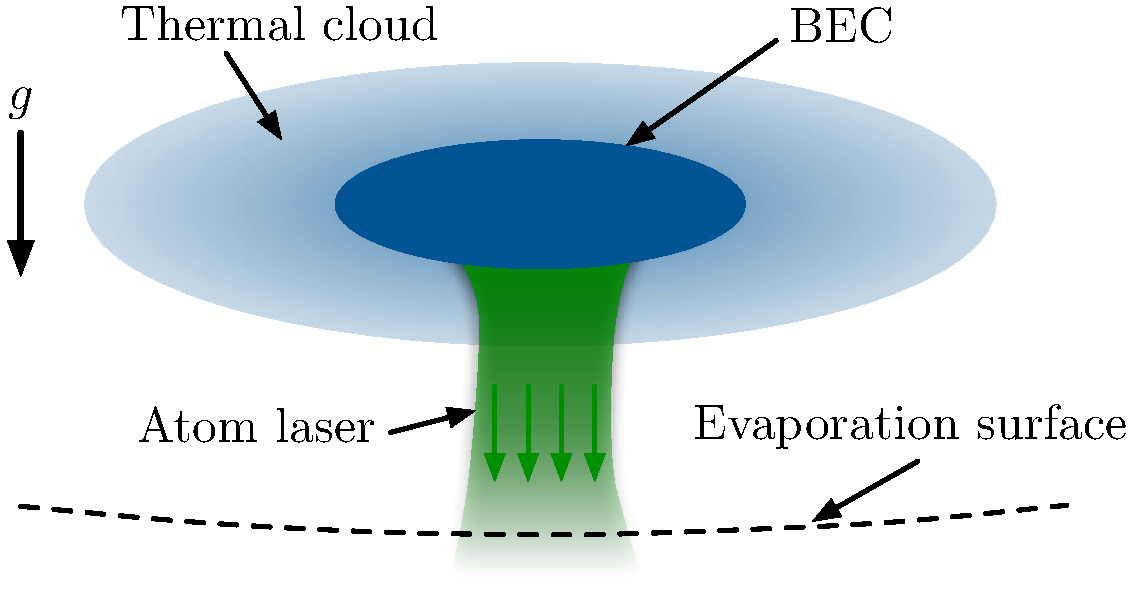
\includegraphics[width=10cm]{QKTScheme}
    \caption{Schematic of the experimental setup. FIXME: Caption.}
    \label{KineticTheory:QKTScheme}
\end{figure}

The proposed scheme for a pumped atom laser is illustrated in \figureref{KineticTheory:QKTScheme}. Bose-enhanced scattering between the thermal atoms and the condensate drives atoms into the condensate. This process becomes irreversible when one of the scattered atoms has enough energy to cross the evaporation surface and be removed from the thermal cloud. The thermal cloud is continuously replenished from a source of atoms at some temperature $T$. The atom laser is produced by large momentum-transfer Raman outcoupling from the condensate to minimise the loss from the atom laser as it traverses the evaporation surface\footnote{An alternative configuration would be to place the evaporation surface \emph{above} the thermal cloud, however the magnetic trap would need to be weak enough for the evaporation surface to be a large distance away from the centre of the magnetic trap. For a trapping frequency of $\omega = 2\pi \times \unit[100]{Hz}$ in the vertical direction, the separation between the centre of the condensate and the centre of the magnetic trap is $y_\text{sag} = \unit[25]{\micro m}$. In such traps, typical condensate sizes are $y_\text{TF} \sim \unit[10]{\micro m}$, not giving much space between the condensate and the thermal cloud. The effectiveness of the evaporation surface is reduced as its size is reduced. For this reason the evaporation surface in \figureref{KineticTheory:QKTScheme} has been pictured below the thermal cloud. FIXME: Rewrite last part of this footnote.}. Using large momentum-transfer Raman outcoupling also minimises the losses from the thermal cloud due to the outcoupling process itself.

FIXME: Rewrite this paragraph as it starts with a statement that seems empty. In order to have net gain into the BEC mode while adding uncondensed atoms to the trap, the system must not be allowed to reach thermal equilibrium. If the thermal cloud is replenished from a source and the radio frequency `scalpel' that produces the forced evaporation is tuned so that atoms of energy $\varepsilon_\text{cut}$ and higher are rapidly and continually removed from the trap, then the condensate will continually experience gain and loss as though it was in the middle of an evaporative step. As $\varepsilon_\text{cut}$ is lowered, a larger fraction of the scattering processes that leave atoms in the condensate mode become irreversible. This suggests that there must be some value of $\varepsilon_\text{cut}$ for which the condensate experiences net gain. What is not clear is whether the net gain can proceed efficiently, i.e. on a timescale much shorter than other losses from the condensate. Lowering $\varepsilon_\text{cut}$ also reduces the total number of thermal atoms present. In the limit that $\varepsilon_\text{cut}$ reaches the condensate energy, there will be no background gas at all, and the condensate cannot experience net gain. We therefore expect that for a given set of parameters, there will be an optimal value for $\varepsilon_\text{cut}$ that maximises the net gain, which may or may not be positive. In order to examine this issue, we have employed quantum kinetic theory (QKT) \citep{Gardiner:1997tz,Jaksch:1997ug,Gardiner:1998wx,Jaksch:1998sj,Gardiner:2000ug,Lee:2000vs,Davis:2000vn}, which has been effective in describing the growth of condensates \citep{Davis:2000vn}.


\section{Model}
\label{KineticTheory:Model}

\begin{figure}
    \centering
        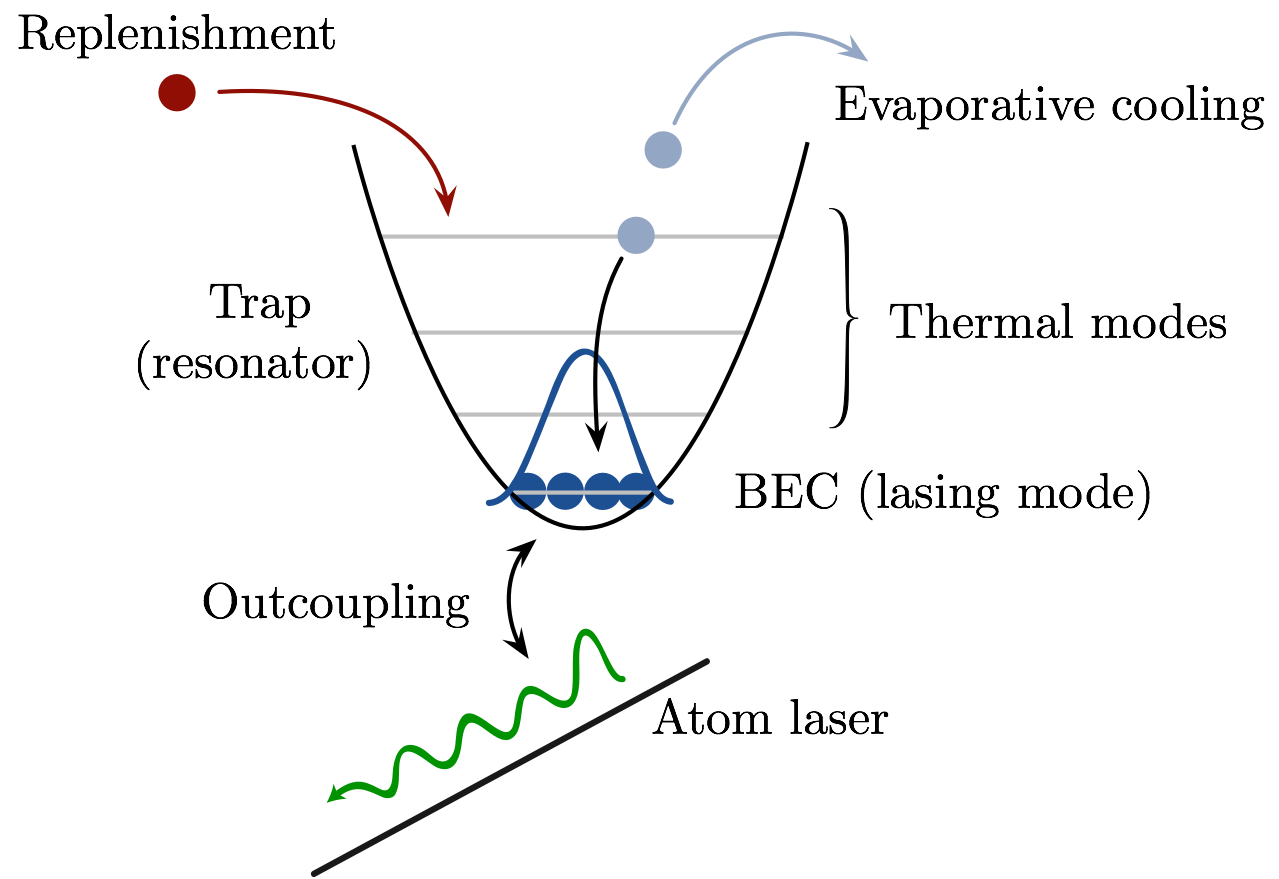
\includegraphics[width=10cm]{QKTModel2}
    \caption{Schematic of the theoretical model. FIXME: Caption.}
    \label{KineticTheory:QKTModel}
\end{figure}

The theoretical model described in this section is an extension of the kinetic model described in \citet{Bijlsma:2000}, which has been successfully used to describe condensate growth. In this section, the model presented in \citep{Bijlsma:2000} is extended to include the replenishment and outcoupling processes illustrated in \figureref{KineticTheory:QKTScheme}. The effect of three-body recombination (the dominant loss process in typical BEC experiments\footnote{FIXME: Cite something.}) is also included. As will be shown later, the inclusion of three-body loss is crucial obtaining a realistic model of the proposed experiment.

The starting point of QKT is to treat separately the thermal and condensed components of the system in \figureref{KineticTheory:QKTScheme}. The condensate is assumed to be adiabatically-evolving and well-described by a Thomas-Fermi distribution. The condensate dynamics are then fully described by the number of atoms in the condensate $N_0(t)$. The thermal cloud is assumed to be well described within the Hartree-Fock approximation as being single particles in the effective potential of the harmonic trap plus condensate mean field. This thermal cloud is then described by its energy distribution function $g(\varepsilon, t)$ and the density of states $\rho(\varepsilon, t)$. The time-dependence of the density of states comes from the inclusion of the effect of the mean field of the condensate on the thermal atoms. The density of states is then fully determined by the trap geometry and the condensate number $N_0(t)$.

The equations of motion for the model can be written in the following form, separating the contributions of the processes involved,
\begin{align}
    \frac{d N_0}{d t} =\begin{split}
        &\relphantom{+}\left. \frac{d N_0}{d t}\right|_\text{thermal--condensate} \\
        &+\left. \frac{d N_0}{d t}\right|_\text{3-body loss} \\
        &+\left. \frac{d N_0}{d t}\right|_\text{outcoupling}
    \end{split},
    & \frac{\partial (\rho g)}{\partial t} = \begin{split}
        &\relphantom{+}\left. \frac{\partial (\rho g)}{\partial t}\right|_\text{thermal--thermal} \\
        &+\left. \frac{\partial (\rho g)}{\partial t}\right|_\text{thermal--condensate} \\
        &+\left. \frac{\partial (\rho g)}{\partial t}\right|_\text{3-body loss} \\
        &+\left. \frac{\partial (\rho g)}{\partial t}\right|_\text{replenishment} \\
        &+\left. \frac{\partial (\rho g)}{\partial t}\right|_\text{redistribution}
    \end{split},
    \label{KineticTheory:EvolutionEquations}
\end{align}
where the subscripts `thermal--thermal' and `thermal--condensate' denote collisional processes between atoms in the corresponding states (\figureref{KineticTheory:ProcessDiagrams}(a) and (b), respectively), the subscript `3-body loss' indicates the contribution due to three-body recombination processes, the subscript `replenishment' indicates the contribution due to the replenishment of the thermal cloud (\figureref{KineticTheory:ProcessDiagrams}(d)), the subscript `outcoupling' indicates the contribution due to outcoupling from the condensate to form the atom laser (\figureref{KineticTheory:ProcessDiagrams}(e)), and the subscript `redistribution' indicates the contribution due to the redistribution of energy levels due to changes in the mean-field of the condensate. 

\begin{figure}
    \centering
    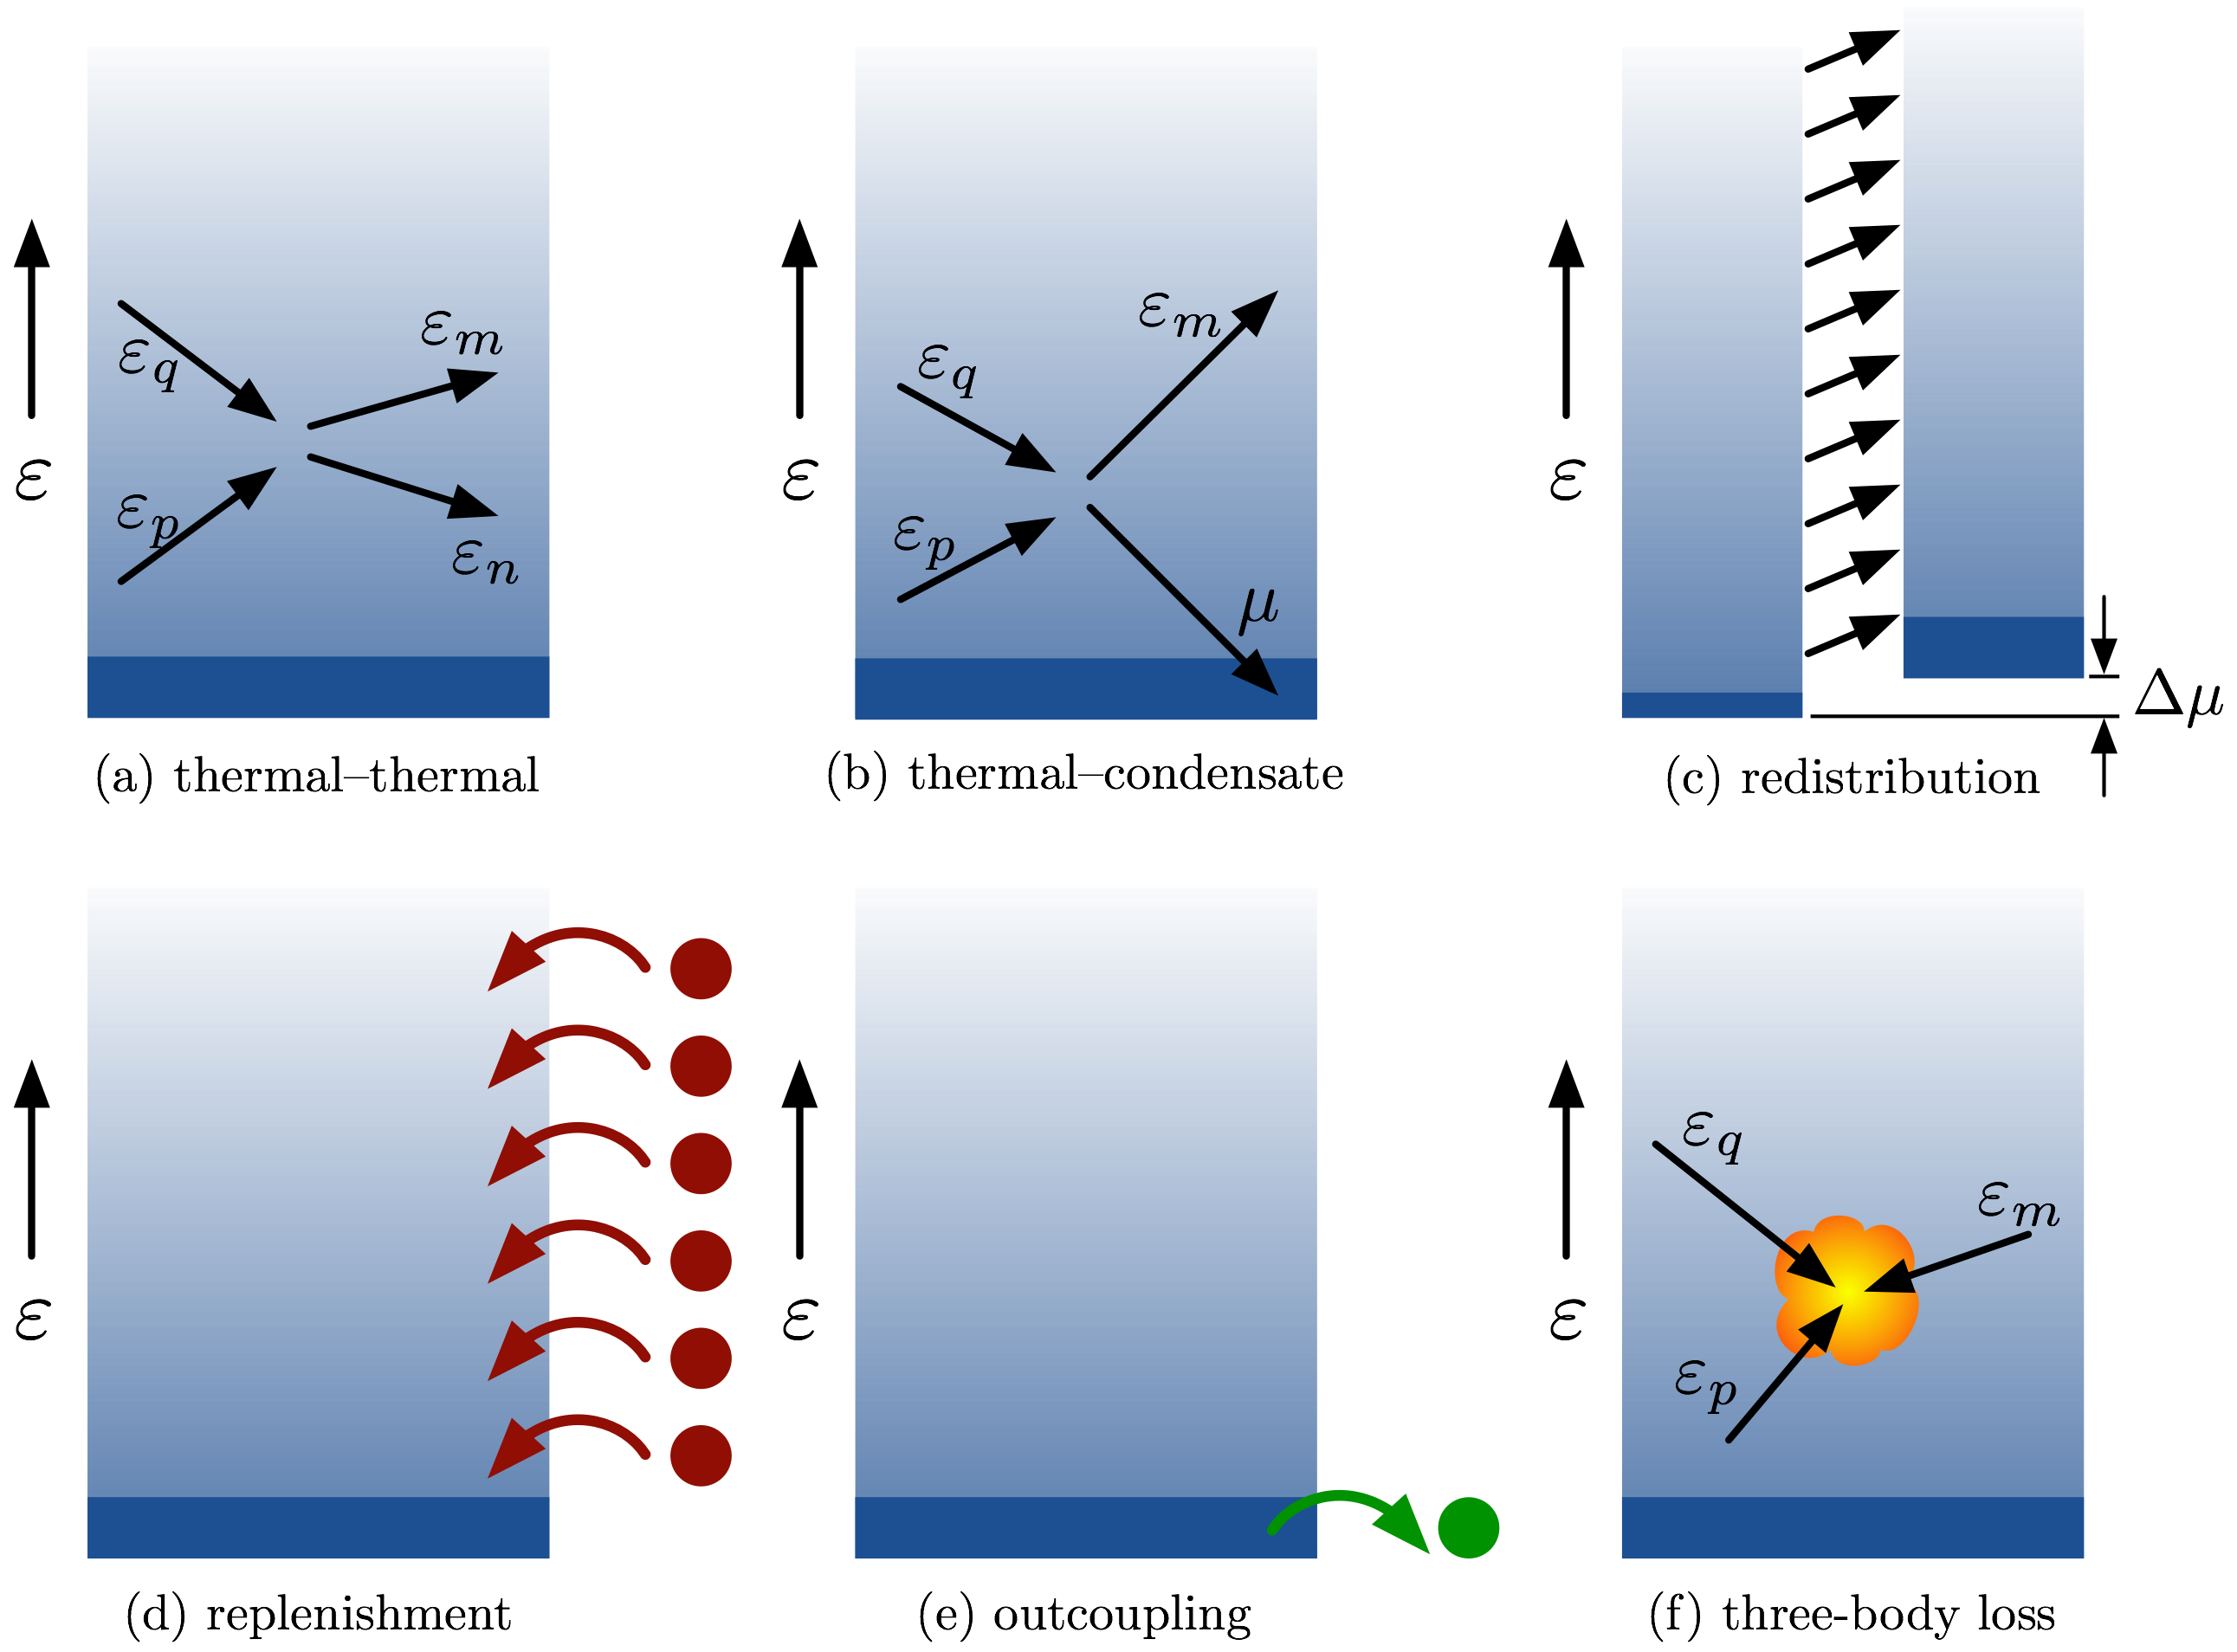
\includegraphics[width=14cm]{ProcessDiagrams}
    \caption{Schematic of the primary processes involved in the evolution of the model described in \eqref{KineticTheory:EvolutionEquations}. The bottom rectangle represents the condensate at $\varepsilon = \mu(t)$. FIXME: Caption.}
    \label{KineticTheory:ProcessDiagrams}
\end{figure}

Derivations of the `thermal--thermal', `thermal--condensate' and `redistribution' terms in \eqref{KineticTheory:EvolutionEquations} are given in \citep{Bijlsma:2000}. The outcoupling process from the condensate is modelled as a simple linear loss process with corresponding rate constant $\gamma$,
\begin{align}
    \left.\frac{d N_0}{d t}\right|_\text{outcoupling} &= - \gamma N_0.
\end{align}
The thermal cloud is modelled as being continuously replenished from a source that provides a constant flux $\Phi$ of atoms at a temperature $T$. For simplicity it is assumed that each energy level $\varepsilon$ in the source is coupled directly to the level in the thermal cloud with energy $\varepsilon + \mu(t)$, i.e. the lowest energy level of the source ($\varepsilon=0$) is coupled directly to the lowest energy level in the trap ($\varepsilon = \mu(t)$). This simple model gives the form of the contribution due to replenishment as
\begin{align}
    \left. \frac{\partial \big(\rho(\varepsilon, t) g(\varepsilon, t))}{\partial t} \right|_\text{replenishment} &= \Phi \rho_0(\varepsilon - \mu(t)) g_T(\varepsilon - \mu(t)),
\end{align}
where $\rho_0(\varepsilon)$ is the density of states in the absence of a condensate, and $g_T(\varepsilon)$ is the Bose-Einstein energy distribution at temperature $T$. The derivation of the contributions to \eqref{KineticTheory:EvolutionEquations} due to three body loss were performed by \emph{Matthew Davis}, and are covered in \sectionref{MethodsAppendix:QKT3BodyLoss}.
%While this is perhaps an unreasonable assumption, it means that we can easily determine the steady state of the system.

FIXME: Write and clean up this paragraph. In obtaining this model a number of assumptions are made:
\begin{enumerate}[(i)]
    \item Ergodic
    \item Adiabatic evolution of the condensate. This also applies at the evaporation cutoff.
    \item Neglect of the anomalous density
    \item Energy scales are such that all non-condensate excitations are particle-like not phonon-like (use of Hartree-Fock mean-field).
\end{enumerate}
These approximations are discussed at length in a comprehensive review article \citep{Proukakis:2008} in which the QKT formalism is referred to as the `ZNG' theory.

The computer code used to solve \eqref{KineticTheory:EvolutionEquations} was written by \emph{Matthew Davis}.

\section{Results}
\label{KineticTheory:Results}
This is my contribution. Example simulations demonstrating time-dependence of the distributions, the dependence on $\eta$. Behaviour (and simple model) in the absence of three-body loss and why this is both obvious and unrealistic. Behaviour (and simple model in high-temperature limit) in the presence of three-body loss.

Joe has suggested that we not rely on the high-temperature limit, but I would really, really like to have that in.

We need a plan for the story that goes in this chapter. This story, and the accompanying graphs are what will be needed to construct the poster for FINESS.

Somewhere we list the full parameters of the model, $T$, $\Phi$, $\gamma$ and $\varepsilon_\text{cut} = \eta k_B T$.

\subsection{Typical results and parameter dependence}
Here we illustrate the time-dependence of a typical solution, and consider the dependence on each parameter. The dependence on most are trivial; only $\eta$ is non-trivial.


\subsection{Behaviour in the absence of three-body loss}
We have a simple model in this case. This model demonstrates that increasing the number of atoms without loss leads to an unbounded increase in the condensation temperature. I'm tempted to not include this discussion in full detail as the entire argument can be given rather concisely just referring to critical temperature, etc.


\subsection{Behaviour in the presence of three-body loss}

\section{Conclusion}
Thermal sources must be close to degenerate to be useful. 